
\documentclass{Configuration_Files/PoliMi3i_thesis}

%------------------------------------------------------------------------------
%	REQUIRED PACKAGES AND  CONFIGURATIONS
%------------------------------------------------------------------------------

% CONFIGURATIONS
\usepackage{parskip} % For paragraph layout
\usepackage{setspace} % For using single or double spacing
\usepackage{emptypage} % To insert empty pages
\usepackage{multicol} % To write in multiple columns (executive summary)
\setlength\columnsep{15pt} % Column separation in executive summary
\setlength\parindent{0pt} % Indentation
\raggedbottom  

% PACKAGES FOR TITLES
\usepackage{titlesec}
% \titlespacing{\section}{left spacing}{before spacing}{after spacing}
\titlespacing{\section}{0pt}{3.3ex}{2ex}
\titlespacing{\subsection}{0pt}{3.3ex}{1.65ex}
\titlespacing{\subsubsection}{0pt}{3.3ex}{1ex}
\usepackage{color}

% PACKAGES FOR LANGUAGE AND FONT
\usepackage[utf8]{inputenc} % UTF8 encoding
\usepackage[T1]{fontenc} % Font encoding
\usepackage[11pt]{moresize} % Big fonts

% PACKAGES FOR IMAGES
\usepackage{graphicx}
\usepackage{transparent} % Enables transparent images
\usepackage{eso-pic} % For the background picture on the title page
\usepackage{subfig} % Numbered and caption subfigures using \subfloat.
\usepackage{tikz} % A package for high-quality hand-made figures.
\usetikzlibrary{}
\graphicspath{{./Images/}} % Directory of the images
\usepackage{caption} % Coloured captions
\usepackage{xcolor} % Coloured captions
\usepackage{amsthm,thmtools,xcolor} % Coloured "Theorem"
\usepackage{float}
\usepackage{listings}

% STANDARD MATH PACKAGES
\usepackage{amsmath}
\usepackage{amsthm}
\usepackage{amssymb}
\usepackage{amsfonts}
\usepackage{bm}
\usepackage[overload]{empheq} % For braced-style systems of equations.
\usepackage{fix-cm} % To override original LaTeX restrictions on sizes

% PACKAGES FOR TABLES
\usepackage{tabularx}
\usepackage{longtable} % Tables that can span several pages
\usepackage{colortbl}

% PACKAGES FOR ALGORITHMS (PSEUDO-CODE)
\usepackage{algorithm}
\usepackage{algorithmic}

% PACKAGES FOR REFERENCES & BIBLIOGRAPHY
\usepackage[colorlinks=true,linkcolor=black,anchorcolor=black,citecolor=black,filecolor=black,menucolor=black,runcolor=black,urlcolor=black]{hyperref} % Adds clickable links at references
\usepackage{cleveref}
\usepackage[square, numbers, sort&compress]{natbib} % Square brackets, citing references with numbers, citations sorted by appearance in the text and compressed
\bibliographystyle{abbrvnat} % You may use a different style adapted to your field

% OTHER PACKAGES
\usepackage{pdfpages} % To include a pdf file
\usepackage{afterpage}
\usepackage{lipsum} % DUMMY PACKAGE
\usepackage{fancyhdr} % For the headers
\fancyhf{}

% Input of configuration file. Do not change config.tex file unless you really know what you are doing. 
% Define blue color typical of polimi
\definecolor{bluepoli}{cmyk}{0.4,0.1,0,0.4}

% Custom theorem environments
\declaretheoremstyle[
  headfont=\color{bluepoli}\normalfont\bfseries,
  bodyfont=\color{black}\normalfont\itshape,
]{colored}

% Set-up caption colors
\captionsetup[figure]{labelfont={color=bluepoli}} % Set colour of the captions
\captionsetup[table]{labelfont={color=bluepoli}} % Set colour of the captions
\captionsetup[algorithm]{labelfont={color=bluepoli}} % Set colour of the captions

\theoremstyle{colored}
\newtheorem{theorem}{Theorem}[chapter]
\newtheorem{proposition}{Proposition}[chapter]

% Enhances the features of the standard "table" and "tabular" environments.
\newcommand\T{\rule{0pt}{2.6ex}}
\newcommand\B{\rule[-1.2ex]{0pt}{0pt}}

% Pseudo-code algorithm descriptions.
\newcounter{algsubstate}
\renewcommand{\thealgsubstate}{\alph{algsubstate}}
\newenvironment{algsubstates}
  {\setcounter{algsubstate}{0}%
   \renewcommand{\STATE}{%
     \stepcounter{algsubstate}%
     \Statex {\small\thealgsubstate:}\space}}
  {}

% New font size
\newcommand\numfontsize{\@setfontsize\Huge{200}{60}}

% Title format: chapter
\titleformat{\chapter}[hang]{
\fontsize{50}{20}\selectfont\bfseries\filright}{\textcolor{bluepoli} \thechapter\hsp\hspace{2mm}\textcolor{bluepoli}{|   }\hsp}{0pt}{\huge\bfseries \textcolor{bluepoli}
}

% Title format: section
\titleformat{\section}
{\color{bluepoli}\normalfont\Large\bfseries}
{\color{bluepoli}\thesection.}{1em}{}

% Title format: subsection
\titleformat{\subsection}
{\color{bluepoli}\normalfont\large\bfseries}
{\color{bluepoli}\thesubsection.}{1em}{}

% Title format: subsubsection
\titleformat{\subsubsection}
{\color{bluepoli}\normalfont\large\bfseries}
{\color{bluepoli}\thesubsubsection.}{1em}{}

% Shortening for setting no horizontal-spacing
\newcommand{\hsp}{\hspace{0pt}}

\makeatletter
% Renewcommand: cleardoublepage including the background pic
\renewcommand*\cleardoublepage{%
  \clearpage\if@twoside\ifodd\c@page\else
  \null
  \AddToShipoutPicture*{\BackgroundPic}
  \thispagestyle{empty}%
  \newpage
  \if@twocolumn\hbox{}\newpage\fi\fi\fi}
\makeatother

%For correctly numbering algorithms
\numberwithin{algorithm}{chapter}

\usepackage{ifxetex}
\usepackage{ifluatex}
\newif\ifxetexorluatex % a new conditional starts as false
\ifnum 0\ifxetex 1\fi\ifluatex 1\fi>0
\xetexorluatextrue
\fi

\ifxetexorluatex
\usepackage{fontspec}
\else
\usepackage[T1]{fontenc}
\usepackage[utf8]{inputenc}
\usepackage[lighttt]{lmodern}
\fi

\usepackage{textcomp}
\usepackage{xcolor}
\usepackage{listings}
\usepackage{upquote}

\definecolor{keyword}{HTML}{2771a3}
\definecolor{pattern}{HTML}{b53c2f}
\definecolor{string}{HTML}{be681c}
\definecolor{relation}{HTML}{7e4894}
\definecolor{variable}{HTML}{107762}
\definecolor{comment}{HTML}{8d9094}
\definecolor{backcolour}{rgb}{0.95,0.95,0.92}

\lstset{
    backgroundcolor=\color{backcolour},
    numbers=none,
    stepnumber=1,
    numbersep=5pt,
    basicstyle=\small\ttfamily,
    keywordstyle=\color{keyword}\bfseries\ttfamily,
    commentstyle=\color{comment}\ttfamily,
    stringstyle=\color{string}\ttfamily,
    identifierstyle=,
    showstringspaces=false,
    aboveskip=3pt,
    belowskip=3pt,
    columns=flexible,
    keepspaces=true,
    breaklines=true,
    captionpos=b,
    tabsize=2,
    frame=none,
}

\lstset{upquote=true}

\lstdefinelanguage{cypher}
{
    morekeywords={
    MATCH, ON, OPTIONAL, WHERE, NOT, AND, OR, XOR, RETURN, DISTINCT, ORDER, BY, ASC, ASCENDING, DESC, DESCENDING, UNWIND, AS, UNION, WITH, ALL, CREATE, DELETE, DETACH, REMOVE, SET, MERGE, SET, SKIP, LIMIT, IN, CASE, WHEN, THEN, ELSE, END,
    INDEX, DROP, UNIQUE, CONSTRAINT, EXPLAIN, PROFILE, START, COUNT, IS, NULL
}
}


\newcommand{\mycdots}{\cdot\!\cdot\!\cdot}
\lstset{language=cypher,
    literate=*
        {...}{$\mycdots$}{1}
        {theta}{$\theta$}{1}
}

%----------------------------------------------------------------------------
%	NEW COMMANDS DEFINED
%----------------------------------------------------------------------------

% EXAMPLES OF NEW COMMANDS
\newcommand{\bea}{\begin{eqnarray}} % Shortcut for equation arrays
\newcommand{\eea}{\end{eqnarray}}
\newcommand{\e}[1]{\times 10^{#1}}  % Powers of 10 notation

%----------------------------------------------------------------------------
%	ADD YOUR PACKAGES (be careful of package interaction)
%----------------------------------------------------------------------------

%----------------------------------------------------------------------------
%	ADD YOUR DEFINITIONS AND COMMANDS (be careful of existing commands)
%----------------------------------------------------------------------------

%----------------------------------------------------------------------------
%	BEGIN OF YOUR DOCUMENT
%----------------------------------------------------------------------------

\begin{document}

\fancypagestyle{plain}{%
\fancyhf{} % Clear all header and footer fields
\fancyhead[RO,RE]{\thepage} %RO=right odd, RE=right even
\renewcommand{\headrulewidth}{0pt}
\renewcommand{\footrulewidth}{0pt}}

%----------------------------------------------------------------------------
%	TITLE PAGE
%----------------------------------------------------------------------------

\pagestyle{empty} % No page numbers
\frontmatter % Use roman page numbering style (i, ii, iii, iv...) for the preamble pages

\puttitle{
	title=SMBUD Project - Neo4j,
	name1=Gabriele Ginestroni, % Author Name and Surname
	name2=Giacomo Gumiero,
	name3=Lorenzo Iovine,
	name4=Nicola Landini,
	name5=Francesco Leone,
	academicyear=2022-2023,
	groupnumber=10
} % These info will be put into your Title page 

%----------------------------------------------------------------------------
%	PREAMBLE PAGES: ABSTRACT (inglese e italiano), EXECUTIVE SUMMARY
%----------------------------------------------------------------------------
\startpreamble
\setcounter{page}{1} % Set page counter to 1

%----------------------------------------------------------------------------
%	LIST OF CONTENTS/FIGURES/TABLES/SYMBOLS
%----------------------------------------------------------------------------

% TABLE OF CONTENTS
\thispagestyle{empty}
\tableofcontents % Table of contents 
\thispagestyle{empty}
\cleardoublepage

\addtocontents{toc}{\vspace{2em}} % Add a gap in the Contents, for aesthetics
\mainmatter % Begin numeric (1,2,3...) page numbering

\chapter{Introduction}
\label{ch:introduction}%
% The \label{...}% enables to remove the small indentation that is generated, always leave the % symbol.

In this chapter will be presented the problem specification and the hypothesis under which the database is implemented.

\section{Problem Specification}
\label{sec:prob_specs}
This project aims to build a graph database that handles scientific articles contained in the DBLP bibliography.
The focus is on creating a database which allows efficient information retrieval from the publications citation network.
The main features analyzed are: articles, authors, venues, fields of study and the relations between all of them.

\section{Assumptions}
\label{sec:assumptions}
\begin{enumerate}
    \item Data in the sources are heterogeneous and can be inconsistent
    \item It is possible that an author writes for different organizations
    \item Field \emph{\_id} in \textbf{author} exists and it is unique
    \item Field \emph{\_id} in \textbf{article} exists and it is unique
    \item It is possible to find a self-reference in a publication
    \item Venues with \emph{type=0} are Conference
    \item Venues with \emph{type=1} are Journal
    \item There is no constraint between the publication type and the venue type in which it is published
\end{enumerate}

\chapter{ER Diagram}
\begin{figure}[H]
    \centering
    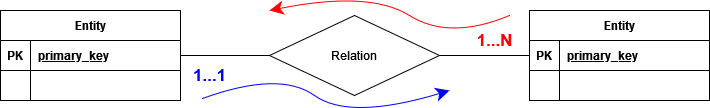
\includegraphics[width=0.6\textwidth]{legendaER.png}
    \caption{ER Diagram Organization}
    \label{fig:erleg}
\end{figure}
\bigskip
\begin{figure}[H]
    \centering
    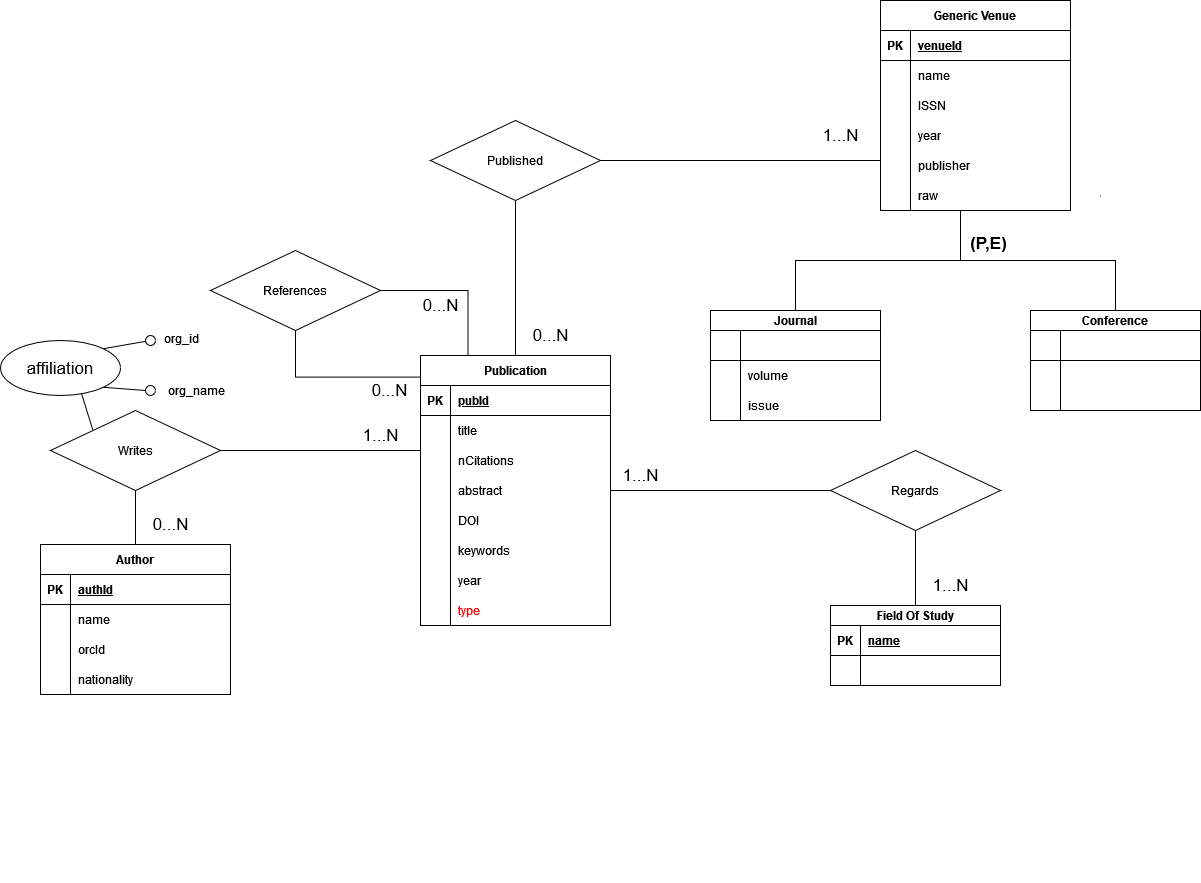
\includegraphics[width=1\textwidth]{ER.png}
    \caption{ER Diagram}
    \label{fig:er}
\end{figure}

\newpage
The ER diagram designed contains the following entities:
\begin{itemize}
    \item \textbf{Publication:} this entity represents all the scientific articles. They are identified by their key \emph{pubId}.
            Other important attributes are: \emph{title, nCitations, abstract, DOI, keywords, year}.
            Publication entity is the superclass of a Total and Exclusive ISA hierarchy with the following subclasses:
            \emph{Journal article, Conference \& Workshop paper, Informal publication, Thesis, Book}.
    \item \textbf{Author:} it is the one who contributed to a publication. Its key is \emph{authId} and its attributes are: \emph{name, orcid, nationality}.
    \item \textbf{Venue:} it is where a publication is published or presented. This is a superclass of a Partial and Exclusive
            ISA hierarchy with the two subclasses \emph{Journal} and \emph{Conference}.
            The key is \emph{venueId} and its other attributes are: \emph{name, ISSN, year, publisher, raw}.
    \item \textbf{Field Of Study:} this entity represents the subjects of the publication and its key is \emph{name}.
\end{itemize}
\bigskip

The ER diagram designed contains the following relationships:
\begin{itemize}
    \item \textbf{Writes:} is the relationship between \emph{author} and \emph{publication} which features the affiliation property
            characterized by org\_id and the org\_name. The affiliation is the institute where the author worked for the publication.
    \item \textbf{References:} is the relationship between a \emph{publication} and another \emph{publication} cited by the first.
    \item \textbf{Regards:} is the relationship between a \emph{publication} and its \emph{fields of study}.
    \item \textbf{Published:} is the relationship between a \emph{publication} and its \emph{venue}.
\end{itemize}

\section{Important differences between ER and the implementation}
\begin{itemize}
    \item As it will be explained in the section 3.2.3, in the implementation we decided to distinguish between different venue
            nodes using the \emph{raw} property. In this way we needed to move some venue attributes (volume, issue, publisher, issn, online\_issn)
            to the relationship \emph{Published}. This has been done due to the low data quality of the dataset with respect to the venue entity.
    \item The publication hierarchy has not been implemented because the dataset used doesn't distinguish between different types of
            publications. We decided to represent the conceptual ER in this way taking inspiration from the DBLP.org site description.
    \item Some attributes that have been included in the ER are missing in the implementation because either not relevant from queries
            point of view or dataset is missing those properties (e.g. \emph{nationality} in \emph{Author}).
\end{itemize}

\chapter{Dataset Description}

\section{Dataset Preprocessing}
The dataset we used is based on DBLP-Citation-network V13 at \url{https://www.aminer.org/citation} whose size is 17GB. Using
\textbf{Pandas Profiling} we analyzed the dataset focusing our attention on distinctness and completeness of the attributes.
We used this result for selecting the property to be used during the merge operation (i.e. attributes with high values of distinctness
and low missing values), to ignore fields that were not informative, and also to filter the tuples. Then we sliced the entire
dataset obtaining a subset of 16MB. The slicing operation was not performed randomly, in order to avoid a subset of the
dataset containing some publications but none of the publications referenced by them. The working sample of about 6400 publications
was obtained in this way:
\begin{itemize}
    \item first a partition of 20M rows was extracted from the original database so that we started from a pool of 257K articles
        instead of using all the original database of ~5.4M articles, we used 5\% as a partition to speed up the sample generation
        process
    \item then an extract of 4K publications was used as a base, we arbitrarily picked the ones from position 20000 to 24000 of the partition
    \item in the end the ids of those 4K publications were looked up inside our partition to obtain also articles that cited
        them, in order to have sufficient relationships to make different queries
\end{itemize}
The following is a part of the script used for the operation just described:
\lstinputlisting[language=Python]{Code/samplePython.txt}
\bigskip
We decide not to add any data to our dataset to preserve data coherency.

\section{Attributes Description}
In this section we will present all the attributes contained in the original dataset, pointing out which of them are considered or not.

\subsection{Publication}
Publication represent the central concept of the system and contains:
\begin{itemize}
    \item \textbf{\_id} is an alphanumeric string that was used during the merge operation, that's because is unique and
            every nodes has this property.
    \item \textbf{title} represents the title of the publication.
    \item \textbf{authors} is a set of authors.
    \item \textbf{venue} it is where a publication is published or presented.
    \item \textbf{year} represents the year of publication.
    \item \textbf{keywords} is a set containing keywords of the publication.
    \item \textbf{fos} is a set containing the fields of study of the publication.
    \item \textbf{n\_citation} is the number of times that this publication has been mentioned.
    \item \textbf{page\_start} defines the starting page of the publication. This attribute wasn't take into consideration
            because doesn't target the goal of the project.
    \item \textbf{page\_end} defines the last page of the publication. This attribute wasn't take into consideration
            because doesn't target the goal of the project.
    \item \textbf{lang} represents the language of the publication.
    \item \textbf{volume} is the volume of the venue in which the article has been published. This is a property of the \emph{Publication}
            - \emph{Venue} relationship.
    \item \textbf{issue} refers to how many times a periodical has been published during that year.
    \item \textbf{issn} is an identification code of the venue of the publication. This is a property of the \emph{Publication}
    - \emph{Venue} relationship.
    \item \textbf{isbn} is an identification code of the venue of the publication. This attribute wasn't take into consideration.
    \item \textbf{doi} Digital Object Identifier is a persistent and standardized identifier. We didn't use this attribute as a key
                    during the importing phase because a significant amount of publication misses it.
    \item \textbf{pdf} contains a string that links to the publication PDF online. This attribute wasn't take into
            consideration due to the presence of many missing or null values.
    \item \textbf{url} contains a set of links to the publication resources online. This attribute wasn't take into
            consideration because doesn't target the goal of the project.
    \item \textbf{abstract} is a string containing a brief summary of the contents of the paper.
    \item \textbf{references} is a set of ids representing the publications mentioned.
\end{itemize}
\bigskip

\subsection{Author}
The dataset provides the following author fields:
\begin{itemize}
    \item \textbf{\_id} is an alphanumeric string that was used during the merge operation, that's because is unique and
            almost every nodes has this parameter.
    \item \textbf{name} is the name of the author.
    \item \textbf{org} is the name of the organization in which the author worked for a specific publication. It is an attribute
            of the relationship \emph{Writes} described before
    \item \textbf{orgid} is the identifier of the organization in which the author worked for a specific publication. It is an
            attribute of the relationship \emph{Writes} described before
    \item \textbf{gid} is an alternative to the orgid field. This attribute wasn't take into consideration due to the presence of many missing or null values.
    \item \textbf{orgs} is a set of organizations for which the author worked. This attribute wasn't take into  consideration
        due to the presence of many missing or null values
    \item \textbf{email} is the email address of the author. This attribute wasn't take into
            consideration due to the presence of many missing or null values and because doesn't target the goal of the 
            project
    \item \textbf{orcid} Open Researcher and Contributor ID is a unique identifier for authors of scientific articles.
            This attribute is taken into consideration although is not always present.
    \item \textbf{oid} is an identifier for the author. This attribute wasn't take into consideration due to the
            presence of many missing or null values.
    \item \textbf{bio} is a string that describes the author. This attribute wasn't take into consideration due to 
            the presence of many missing or null values.
    \item \textbf{sid} is an identifier for the author. This attribute wasn't take into consideration due to the
            presence of many missing or null values.
    \item \textbf{name\_zh} is a field that describe name in chinese language. This attribute wasn't take
            into consideration due to the presence of many missing or null values.
    \item \textbf{org\_zh} is a field that describe the organization in chinese language. This attribute
            wasn't take into consideration due to the presence of many missing or null values.
\end{itemize}
\bigskip

\subsection{Venue}
Venue is where a publication is published or presented. It contains:
\begin{itemize}
    \item \textbf{\_id} is an alphanumeric identifier. We didn't use this property for the merge operation due to the large
            amount of missing values as previously stated.
    \item \textbf{raw} is the name or the abbreviation of the venue (regardless the year, issue or volume) in which the
            publication was presented. This property was used during the merge operation due to the low number of missing
            values and the fact that in this way publications were grouped based on the name or the abbreviation of the venue in which they were presented.
    \item \textbf{raw\_zh} refers to the event (without specifying the year) in which the publication was presented. 
            This attribute wasn't take into consideration due to the presence of many missing or null values.
    \item \textbf{type} indicates the type of the publication. Exploiting the profiling we understood the distribution
            of different values of \emph{type}, and become clear that 0 and 1 were attributable respectively to conference
            and journal. The other values were not easily attributable to other types of publication, so we decided to consider
            as a generic venue:
            \begin{itemize}
                \item every \emph{type} values different from 0 or 1
                \item every entity in which the \emph{type} field is missing
            \end{itemize} 
    \item \textbf{sid} unclear and frequently missing attribute. This attribute wasn't take into consideration.
    \item \textbf{t} represents the type of the publication. This attribute wasn't take into consideration due to the
            presence of many missing or null values.
    \item \textbf{issn} is an identification code of the venue of the publication. We used the one in Publication instead of
        this one after seeing the profiling results.
    \item \textbf{name\_d} is the extended name of the event or volume in which the publication was presented.
    \item \textbf{publisher} is the name of the publisher of the Venue.
    \item \textbf{online\_issn} is an alternative identification code with respect to the issn. This is a property of the \emph{Publication}
        - \emph{Venue} relationship.
\end{itemize}

\chapter{Graph Diagram}
The designed graph diagram presented on the next page represents the following nodes:
\begin{itemize}
    \item \textbf{Publication}
    \item \textbf{Author}
    \item \textbf{Venue}
    \item \textbf{Field of Study}
\end{itemize}
The properties of the nodes are the ones described in the previous chapter.\\
The diagram also represents the following links:
\begin{itemize}
    \item \textbf{Writes} links \emph{Author} with the \emph{Publication} that he wrote. His properties are \emph{org} and \emph{orgid}
        that represent the institute where the Author worked for that specific publication.
    \item \textbf{Published} links \emph{Publication} with the \emph{Venue} in which it was published. His properties are \emph{issue}, \emph{volume},
        \emph{issn}, \emph{publisher} and \emph{online\_issn}.
    \item \textbf{Regards} links \emph{Publication} with the \emph{Fields of Study}.
    \item \textbf{References} links a \emph{Publication} with another \emph{Publication} it cites.
\end{itemize}
\bigskip
In the following diagram we decided to represent two \emph{Authors}, two \emph{Publications}, two \emph{Fields of Study} and
two \emph{Venues} (one \emph{Journal} and one \emph{Conference}) in order to efficiently describe the system functionalities. \newline
In this case \emph{Author1} wrote both the \emph{Publications}, while the other one wrote only \emph{Publication2}.
Both the \emph{Publications} covered the same \emph{Fields of Study} but \emph{Publication1} was published in a conference,
while the other one was published in a journal. Eventually a relationship \emph{References} that
links \emph{Publication1} with \emph{Publication2} exists meaning that \emph{Publication1} cites \emph{Publication2}.
\begin{figure}[H]
    \centering
    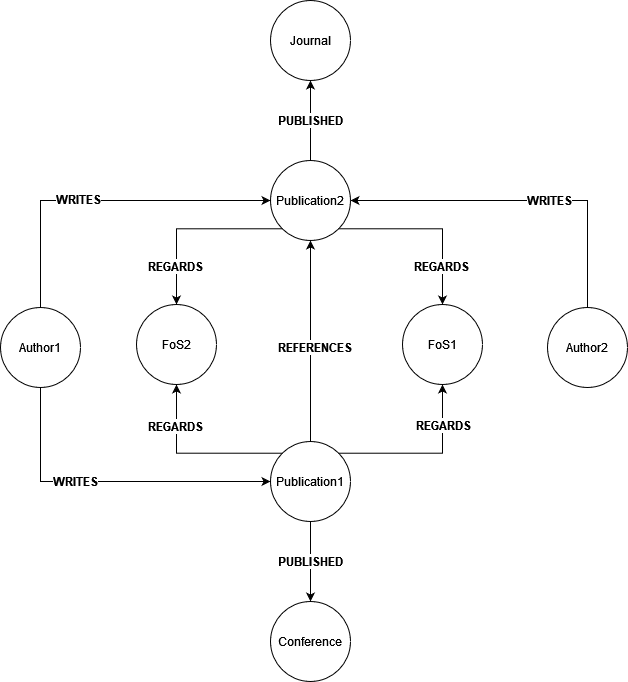
\includegraphics[width=0.6\textwidth]{graphDiagram.png}
    \caption{Graph Diagram}
    \label{fig:graphDiagram}
\end{figure}

\chapter{Sample Dataset}
In this chapter we will present the import commands that generates 39550 nodes distributed as follows:
\begin{itemize}
    \item 6340 \emph{Publication} nodes
    \item 17025 \emph{Author} nodes
    \item 2133 \emph{Conference} nodes
    \item 256 \emph{Journal} nodes
    \item 506 \emph{Generic Value} nodes
    \item 13210 \emph{Field of Study} nodes
\end{itemize}
In order to complete these operations we used the plug-in apoc.

\begin{enumerate}
    \item Create \emph{Publication}, \emph{Author} and \verb |WRITES| relationship between them:
        \begin{lstlisting}[language=cypher, label=lst:cypher-example]
call apoc.load.json("test.json") yield value
UNWIND value AS pub
UNWIND pub.authors AS aut WITH aut,pub WHERE aut._id IS NOT NULL
MERGE (publication:Publication{id:pub._id}) ON CREATE SET
    publication.title  = pub.title,
    publication.doi = pub.doi,
    publication.year = pub.year,
    publication.n_citation = pub.n_citation,
    publication.keywords = pub.keywords,
    publication.abstract = pub.abstract,
    publication.lang = pub.lang
MERGE(author:Author{id:aut._id}) ON CREATE SET
    author.name = aut.name,
    author.orcid = aut.orcid
MERGE(author)-[writes:WRITES]->(publication) ON CREATE SET
    writes.org=aut.org,
    writes.orgid=aut.orgid
        \end{lstlisting}
        Added 23365 labels, created 23365 nodes, set 138863 properties, created 18534 relationships.
    \item Create \verb |REFERENCE| relationship between \emph{Articles}:
        \begin{lstlisting}[language=cypher, label=lst:cypher-example]
call apoc.load.json("test.json") yield value
UNWIND value AS pub
UNWIND pub.references AS ref
MATCH (init:Publication{id:pub._id})
MATCH (final:Publication{id:ref})
MERGE(init)-[:REFERENCES]->(final)
        \end{lstlisting}
        Created 2866 relationships.
    \item Create \emph{Conference} when \verb |raw| exists and \verb |type| equal to 0:
        \begin{lstlisting}[language=cypher, label=lst:cypher-example]
call apoc.load.json("test.json") yield value
UNWIND value AS art
WITH art WHERE art.venue.raw IS NOT NULL AND art.venue.type = 0
MATCH(article:Publication{id: art._id})
MERGE(venue:Conference{raw:art.venue.raw}) ON CREATE SET
    venue.name = art.venue.name_d
MERGE(article)-[pub:PUBLISHED]->(venue) ON CREATE SET
    pub.issue = art.issue,
    pub.volume = art.volume,
    pub.issn = art.issn,
    pub.online_issn = art.venue.online_issn,
    pub.publisher = art.venue.publisher
        \end{lstlisting}
        Added 2133 labels, created 2133 nodes, set 22676 properties, created 4846 relationships.
    \item Create \emph{Journal} when \verb |raw| exists and \verb |type| equal to 1:
        \begin{lstlisting}[language=cypher, label=lst:cypher-example]
call apoc.load.json("test.json") yield value
UNWIND value AS art
WITH art WHERE art.venue.raw IS NOT NULL AND art.venue.type = 1
MATCH(article:Publication{id:art._id})
MERGE(venue:Journal{raw:art.venue.raw}) ON CREATE SET
    venue.name = art.venue.name_d
MERGE(article)-[pub:PUBLISHED]->(venue) ON CREATE SET
    pub.issue = art.issue,
    pub.volume = art.volume,
    pub.issn = art.issn,
    pub.online_issn = art.venue.online_issn,
    pub.publisher = art.venue.publisher
        \end{lstlisting}
        Added 256 labels, created 256 nodes, set 1681 properties, created 351 relationships.
    \item Create \emph{Generic Venue} when \verb |raw| doesn't exist or \verb |type| different from 0 or 1:
        \begin{lstlisting}[language=cypher, label=lst:cypher-example]
call apoc.load.json("test.json") yield value
UNWIND value AS art
WITH art WHERE art.venue.raw IS NOT NULL AND (art.venue.type IS NULL OR (art.venue.type <> 1 and art.venue.type <> 0))
MATCH(article:Publication{id:art._id})
MERGE(venue:GenericVenue{raw:art.venue.raw}) ON CREATE SET
    venue.name = art.venue.name_d
MERGE(article)-[pub:PUBLISHED]->(venue) ON CREATE SET
    pub.issue = art.issue,
    pub.volume = art.volume,
    pub.issn = art.issn,
    pub.online_issn = art.venue.online_issn,
    pub.publisher = art.venue.publisher
        \end{lstlisting}
        Added 586 labels, created 586 nodes, set 5122 properties, created 1116 relationships.
    \item Create \emph{Field of Study} and \verb |REGARDS| relationship between \emph{FoS} and \emph{Publication}:
        \begin{lstlisting}[language=cypher, label=lst:cypher-example]
call apoc.load.json("test.json") yield value
UNWIND value AS pub
UNWIND pub.fos AS f
MATCH(publication:Publication{id:pub._id})
MERGE(fos:Fos{name:f})
MERGE (publication)-[:REGARDS]->(fos)
        \end{lstlisting}
        Added 13210 labels, created 13210 nodes, set 13210 properties, created 59740 relationships.
\end{enumerate}


\chapter{Commands and Queries}
\section{Commands}
We have identified the following \verb |INSERT| and \verb |UPDATE| commands to show the system basic functionalities.

\subsection{Insert two authors in the system}
Assuming they are not present in the dataset, we used the \verb |CREATE| to create two instances of \emph{Author}.
\begin{lstlisting}[language=cypher, label=lst:cypher-example]
CREATE (author1:Author {id: "54857748dabfae8a11fb2a1e", name: "Emanuele Della Valle", orcid: "0000-0002-5176-5885"})
CREATE (author2:Author {id: "53f487fbdabfaee4dc8b1e68", name: "Alessio Bernardo", orcid: "0000-0002-3492-0345"})
\end{lstlisting}

\subsection{Insert Journal Venue where the paper has been published}
Assuming they are not present in the dataset, we used the \verb |CREATE| to create an instance of \emph{Venue (Journal)}
specifying where it was published.
\begin{lstlisting}[language=cypher, label=lst:cypher-example]
CREATE (journal:Journal {raw: "ESA", name: "Expert Systems with Applications"})
\end{lstlisting}

\subsection{Create (if do not exist) publication's fields of study}
We used the \verb |MERGE| to create three instances of \emph{Field Of Study}
\begin{lstlisting}[language=cypher, label=lst:cypher-example]
MERGE (fos1:Fos{name:"Computer Science"})
MERGE (fos2:Fos{name:"Stream Reasoning"})
MERGE (fos3:Fos{name:"Big Data"})
\end{lstlisting}

\subsection{Create a publication and his relationships with already existing entities}
At the beginning we \verb |MATCH| two specific \emph{Authors}, three specific \emph{Fields of Study} and one specific
\emph{Journal}. Then, we create the \emph{Publication} and the relationships with the entities listed before
\begin{lstlisting}[language=cypher, label=lst:cypher-example]
MATCH (author1:Author),(author2:Author) WHERE author1.id = "54857748dabfae8a11fb2a1e" AND author2.id = "53f487fbdabfaee4dc8b1e68"
MATCH (fos1:Fos),(fos2:Fos),(fos3:Fos) WHERE fos1.name="Computer Science" AND fos2.name="Stream Reasoning" AND fos3.name="Big Data"
MATCH (journal:Journal) WHERE journal.raw = "ESA"
CREATE (pub:Publication{id: "53e99f86b7612d9702859fdf",
    doi: "10.1016/j.eswa.2022.116630",
    title: "An extensive study of C-SMOTE, a Continuous Synthetic Minority Oversampling Technique for Evolving Data Streams",
    year: 2022,
    n_citation: 3,
    keywords: ["Evolving Data Stream","Streaming","Concept drift","Balancing"],
    abstract: "Streaming Machine Learning (SML) studies algorithms that update their models, given an unbounded and often non-stationary flow of data performing a single pass.",
    lang: "en"})

//Creation of relationship WRITES between authors and the article
CREATE (author1)-[:WRITES{org: "Politecnico di Milano",
    orgid: "5b86c975e1cd8e14a3d351a3"}]->(pub),
    (author2)-[:WRITES{org: "Politecnico di Milano",
    orgid: "5b86c975e1cd8e14a3d351a3"}]->(pub)

//Creation of relationship REGARDS between article and fields of study
CREATE (pub)-[:REGARDS]->(fos1),
    (pub)-[:REGARDS]->(fos2),
    (pub)-[:REGARDS]->(fos3)

//Creation of relationship PUBLISHED between the article and the journal
//Note that in this case fields online_issn and issue are not available
CREATE (pub)-[published:PUBLISHED{volume:"196",
    issn: "0957-4174",
    publisher:"Elsevier"}]->(journal)
\end{lstlisting}

\subsection{Create REFERENCES relationship among the article and the cited ones}
We \verb |MATCH| the two publications referred by our article and we create \verb |REFERENCES| relationships that link
the publications already present in the dataset with the article just created
\begin{lstlisting}[language=cypher, label=lst:cypher-example]
MATCH (p1:Publication),(p2:Publication),(p:Publication{id:'53e99f86b7612d9702859fdf'})
WHERE p1.id = "53e99fe4b7602d97028bf743" AND p2.id="53e99fddb7602d97028bc085"
CREATE (p)-[:REFERENCES]->(p1), (p)-[:REFERENCES]->(p2)
\end{lstlisting}

\subsection{Increment cited publications' n\_citation attribute by 1}
It's an update command that increments the number of citations of the two articles cited by the article that we created
in the previous commands
\begin{lstlisting}[language=cypher, label=lst:cypher-example]
MATCH (p1:Publication), (p2:Publication)
WHERE p1.id = "53e99fe4b7602d97028bf743" AND p2.id="53e99fddb7602d97028bc085"
SET p1.n_citation = p1.n_citation + 1, p2.n_citation = p2.n_citation + 1
\end{lstlisting}

\section{Queries}
We have identified the following queries in order to show the system's basic functionalities.

\subsection{Query 1}
This query returns all the venues where have been published the articles of one of the authors that have written the max number of articles\\
\textbf{Description:} for each author we count how many articles he wrote, then we order by the count of written articles by descending order and keep only the top 1 author. 
Eventually we match all the articles written by this author and we return the raw of the venues in which these articles were published
\begin{lstlisting}[language=cypher, label=lst:cypher-example]
MATCH(author:Author)-[:WRITES]->(article:Publication)
WITH author, count(*) AS articleWritten
ORDER BY articleWritten DESC
WITH author AS authorMax, articleWritten LIMIT 1
MATCH(authorMax:Author)-[:WRITES]->(article)
MATCH(article:Publication)-[:PUBLISHED]->(venue)
RETURN DISTINCT venue.raw
\end{lstlisting}
\begin{figure}[H]
\centering
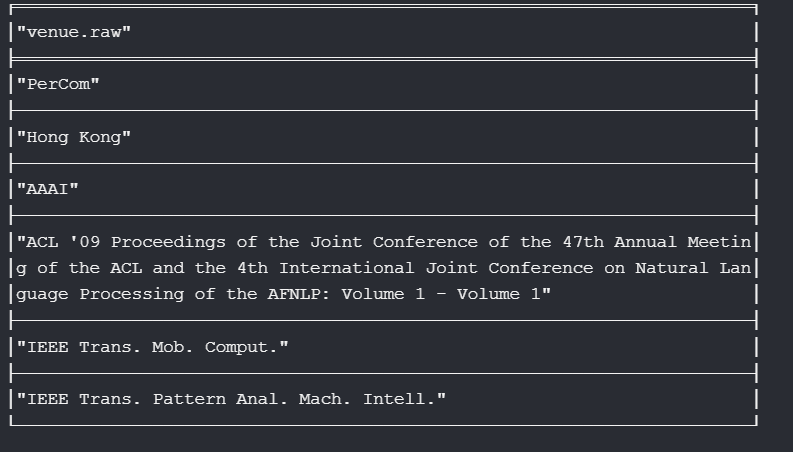
\includegraphics[width=0.6\textwidth]{query/query1.PNG}
\caption{Results: 6 records}
\label{fig:query1}
\end{figure}

\subsection{Query 2}
Starting from the author found in query 1 we want to find the article with the max number of co-authors and return the venue and fields of study\\
\textbf{Description:} we match a specific author given its id, then we match all his articles and then all the co-authors of his articles.
Then, for each article we count the number of co-authors and order them by descending order w.r.t. the number of co-authors.
We keep the top article, then we match its venues and its fields of study and return them by collecting the fos into a list
\begin{lstlisting}[language=cypher, label=lst:cypher-example]
MATCH(author:Author{id:'548d281cdabfae8a11fb4ea1'})
MATCH(author)-[:WRITES]->(article)
MATCH(article)<-[:WRITES]-(coAuth)
WITH article , count(*) AS nCount
ORDER BY nCount DESC LIMIT 1
MATCH(article)-[:PUBLISHED]->(venues)
MATCH(article)-[:REGARDS]->(fos)
RETURN venues.raw AS Venue, collect(fos.name) AS FieldsOfStudy
\end{lstlisting}
\begin{figure}[H]
\centering
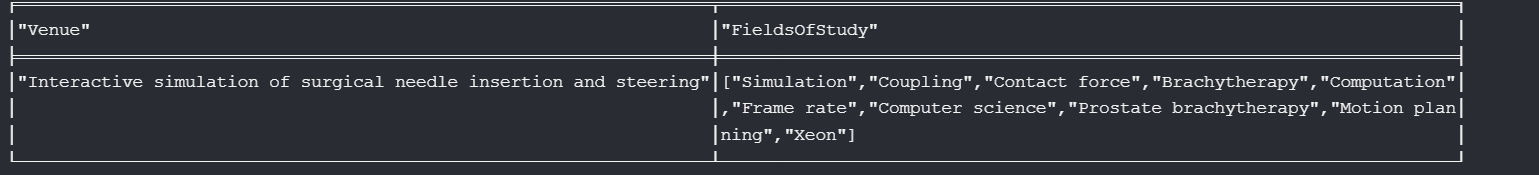
\includegraphics[width=1\textwidth]{query/query2.PNG}
\caption{Result: 1 record}
\label{fig:query2}
\end{figure}

\subsection{Query 3}
This query finds all authors that have worked together more than once on the same field of study\\
\textbf{Description:} we match 2 different authors and 2 different articles in which they collaborated,
matching also all their fields of study, then we filter by keeping only those who have at least one field of study in common.
Eventually we return the name of the two authors\\
\textbf{Note:} the condition on the authors id needed to ensure that every couple is returned only once\\
\textbf{Note:} query result picture is partial
\begin{lstlisting}[language=cypher, label=lst:cypher-example]
MATCH(aut1:Author)-[:WRITES]->(art1)-[:REGARDS]->(fos1)
MATCH(aut1:Author)-[:WRITES]->(art2)-[:REGARDS]->(fos2)
MATCH(aut2:Author)-[:WRITES]->(art1)
MATCH(aut2:Author)-[:WRITES]->(art2)
WHERE (art1)<-[:WRITES]-(aut2) AND
    (art2)<-[:WRITES]-(aut2) AND
    art1.id <> art2.id AND aut1.id > aut2.id
    AND fos1 = fos2
RETURN DISTINCT aut2.name, aut1.name
\end{lstlisting}
\begin{figure}[H]
\centering
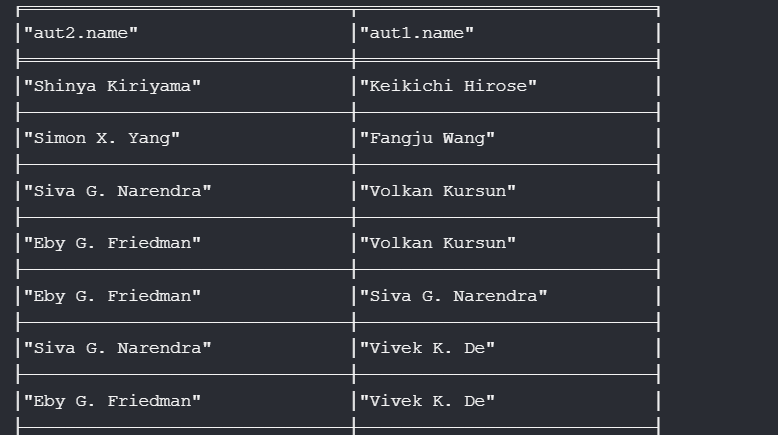
\includegraphics[width=0.6\textwidth]{query/query3.PNG}
\caption{Results: 526 records}
\label{fig:query3}
\end{figure}

\subsection{Query 4}
Find shortest path of WRITES links between an author that wrote a publication for a Stanford University and another author
that wrote an article for a California University.\\
\textbf{Description:} we match 2 authors such that one has published at least once in affiliation with Stanford university and the other with California university.
We check that the 2 authors are not the same and then we compute the shortest path between them (composed of WRITES relationships) bounded to 5 steps.
Then for all the obtained paths we keep the ones with length > 2 to avoid trivial path.\\
\textbf{Note:} graph image is a subset of actual query result (PATH: Kunle ->...-> Krste)
\begin{lstlisting}[language=cypher, label=lst:cypher-example]
MATCH (auth1:Author), (auth2:Author)
WHERE EXISTS {
    MATCH (auth1)-[w:WRITES]->()
    WHERE w.org CONTAINS 'Stanford'}
AND EXISTS {
    MATCH (auth2)-[v:WRITES]->()
    WHERE v.org CONTAINS 'California'}
AND auth1 <> auth2
MATCH p = shortestPath((auth1)-[:WRITES*1..5]-(auth2))
WHERE length(p) > 2
RETURN p, auth1.name, auth2.name
\end{lstlisting}
\begin{figure}[H]
\centering
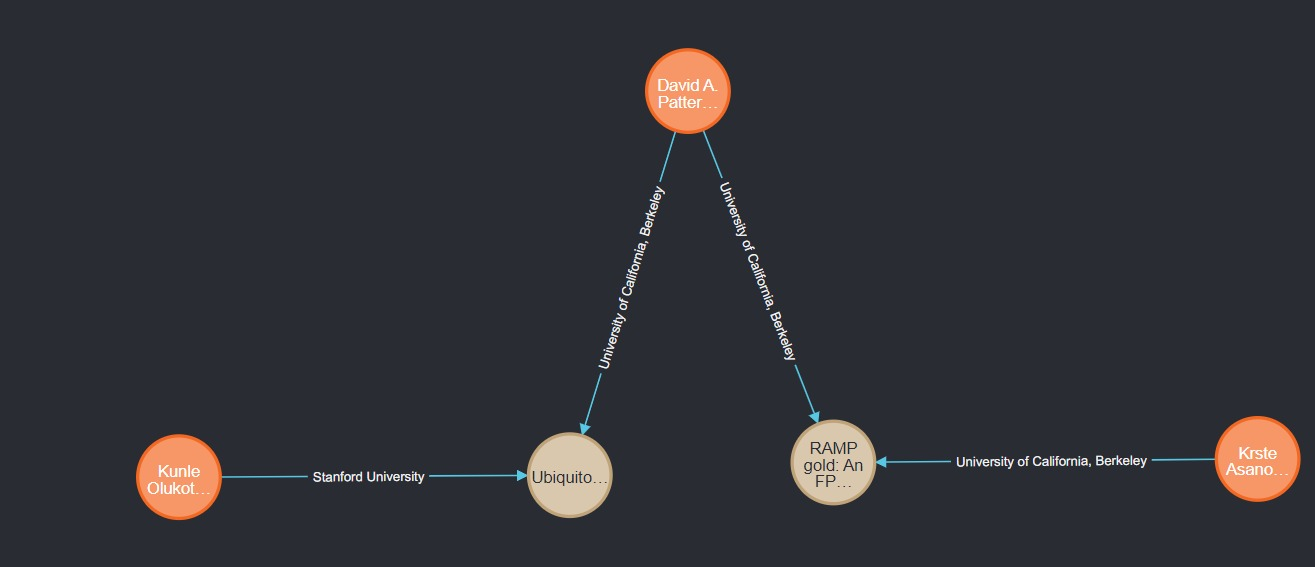
\includegraphics[width=0.7\textwidth]{query/query4.jpeg}
\caption{Results: 18 records, only 1 path in the figure for readability}
\label{fig:query4}
\end{figure}

\subsection{Query 5}
Find the venue with the highest average number of citations of its publications starting from year 1990 and return the most frequent field of study of its publications.\\
\textbf{Description:} we match all the publications that have the year attribute > 1990, then we group with respect to the venue they've been published.
Then for each venue we compute the average of the number of citations of the articles that were published on it.
After that we order the averages by descending order and keep the greatest one. Then we match all the fields of study of all the articles (ignoring the publication date)
that have been published on that venue. After that, we count those fields of study, order by descending order and keep only the most frequent one.
Finally we return the venue, its most frequent field of study and the number of occurrences of that field of study
\begin{lstlisting}[language=cypher, label=lst:cypher-example]
MATCH (v)<-[p:PUBLISHED]-(a:Publication)
WHERE a.year > 1990 AND a.n_citation IS NOT NULL
WITH v, avg(a.n_citation) AS mean, count(a) AS n_article
ORDER BY mean DESC
WHERE n_article > 5
WITH v AS venue, mean, n_article LIMIT 1
MATCH (fos)<-[:REGARDS]-(art)-[:PUBLISHED]->(venue)
WITH fos, count(*) AS fosN, venue
ORDER BY fosN DESC LIMIT 1
RETURN venue.raw AS VenueRaw, fos.name AS FieldOfStudy, fosN AS FieldOfStudyOccurrence
\end{lstlisting}
\begin{figure}[H]
\centering
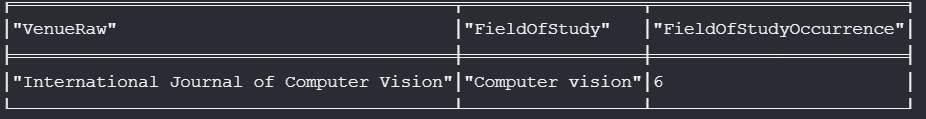
\includegraphics[width=0.7\textwidth]{query/query5.PNG}
\caption{Result: 1 record}
\label{fig:query5}
\end{figure}

\subsection{Query 6}
Find the 3 most common fos (and their count) of the articles published on the volume of \emph{Clinical Orthopaedics and Related Research}
that received the greatest number of total citations.\\
\textbf{Description:} we match the specific journal using the raw, then we aggregate with respect to the volume in which
articles were published and sum their number of citations. Then we order by descending order and keep the 1st volume. Finally,
we match all the relationships with that volume involving the same venue as before, grouping by fields of study and counting
their occurrences. We return the top 3 fields of study according to their count.
\begin{lstlisting}[language=cypher, label=lst:cypher-example]
MATCH (j:Journal{raw:'Clinical Orthopaedics and Related Research'})<-[p:PUBLISHED]-(art)
WITH p.volume as pVolume, sum(art.n_citation) as totalVolumeCitations
ORDER BY totalVolumeCitations DESC LIMIT 1
MATCH (j:Journal{raw:'Clinical Orthopaedics and Related Research'})<-[p:PUBLISHED{volume:pVolume}]-(art)
MATCH (art)-[:REGARDS]->(fos)
WITH fos, count(*) as fosCount
ORDER BY fosCount DESC LIMIT 3
RETURN fos.name as fieldOfStudy,fosCount
\end{lstlisting}
\begin{figure}[H]
\centering
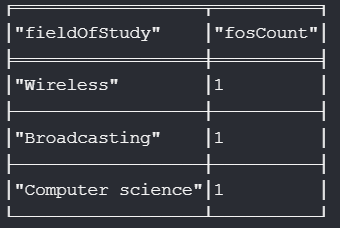
\includegraphics[width=0.3\textwidth]{query/query6.PNG}
\caption{Results: 3 records}
\label{fig:query6}
\end{figure}

\subsection{Query 7}
Find the authors of the article that cites articles with the greatest number of different years of publication.\\
\textbf{Description:} we match in a subquery the \verb |REFERENCES| relationships and return all the article-year(of the
referenced article) pairs. Then, we count for each article all the year values returned by the previous subquery. We
order the articles according to the count in descending order and keep the top one. Then we match the authors of the top
1 article and return their names.
\begin{lstlisting}[language=cypher, label=lst:cypher-example]
CALL {
    MATCH (art1:Publication)-[:REFERENCES]->(art2:Publication)
    RETURN DISTINCT art1 , art2.year AS year
}
WITH art1, count(year) as nCount
ORDER BY nCount DESC LIMIT 1
MATCH (author)-[:WRITES]->(art1)
RETURN COLLECT(author.name) AS authors, nCount
\end{lstlisting}
\begin{figure}[H]
\centering
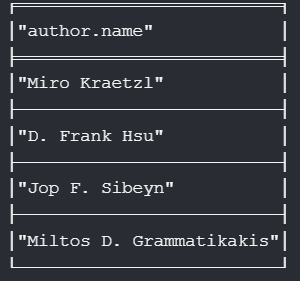
\includegraphics[width=1\textwidth]{query/query7.PNG}
\caption{Results: 1 record}
\label{fig:query7}
\end{figure}

\subsection{Query 8}
Find the authors that have written an article for \emph{Stanford} and an article for another organization.\\
\textbf{Description:} We match for each author 2 publications such that one has been written in affiliation with \emph{Stanford}
and the other one not (the previous condition ensures that the two articles are different). Finally we return the articles'
title and their author name.
\begin{lstlisting}[language=cypher, label=lst:cypher-example]
MATCH (article)<-[w1:WRITES]-(author)-[w2:WRITES]->(article1)
WHERE w1.org CONTAINS "Stanford" AND NOT w2.org CONTAINS "Stanford"
RETURN article1.title,article.title, author.name
\end{lstlisting}
\begin{figure}[H]
\centering
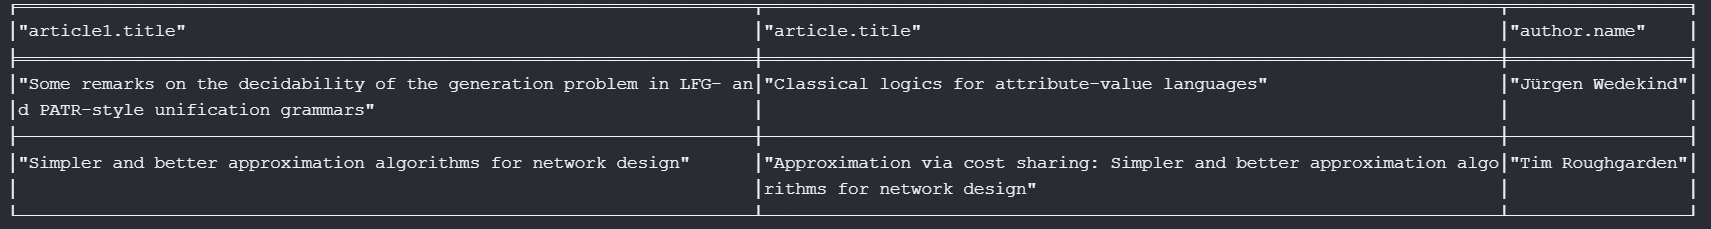
\includegraphics[width=1\textwidth]{query/query8.PNG}
\caption{Results: 2 records}
\label{fig:query8}
\end{figure}

\subsection{Query 9}
Find the shortest path (of length of at least 2) of references between a specific publication and a publication written in
affiliation with \emph{Stanford University}.\\
\textbf{Description:} we match the publication with a specific id and another publication that has been written in
affiliation with \emph{Stanford}. We compute the shortest path of \verb |REFERENCES| relationships connecting them, bounding
the search to 5 steps of depth).
\begin{lstlisting}[language=cypher, label=lst:cypher-example]
MATCH (a:Publication{id:'53e9a0eeb7602d97029d96d3'}),
    (a2:Publication),
    p = shortestPath((a)-[:REFERENCES*1..5]->(a2))
WHERE EXISTS {
    (auth1)-[w:WRITES]->(a2)
    WHERE w.org CONTAINS 'Stanford'
}
AND length(p) > 2
RETURN p
\end{lstlisting}
\begin{figure}[H]
\centering
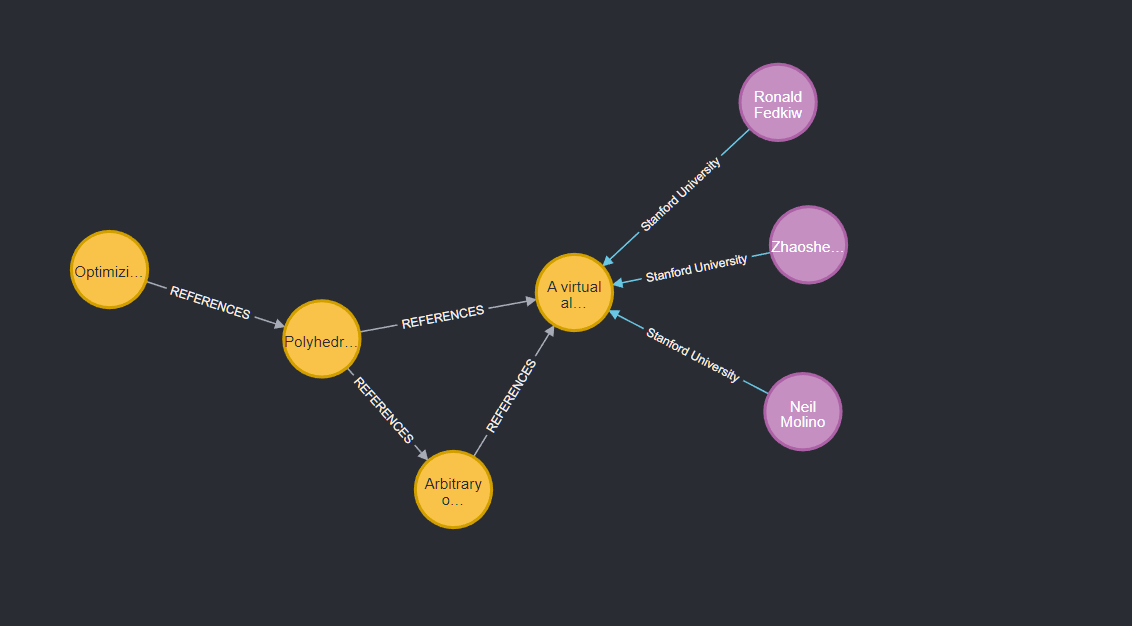
\includegraphics[width=0.6\textwidth]{query/query9.PNG}
\caption{Result: 1 record}
\label{fig:query9}
\end{figure}

\subsection{Query 10}
All articles with venue \verb |SIGIR| written by authors that combined have all 26 letters of the alphabet.\\
\textbf{Description:} We match all the articles published on a specific venue, then we match all the writes relationships
and for each publication we combine all the authors' name letters together and keep the publications where the combined
authors' letters are covering the entire alphabet (case insensitive and ignoring special characters). Finally we return
the publication title and the list of all the authors' names
\begin{lstlisting}[language=cypher, label=lst:cypher-example]
MATCH (art:Publication)-[:PUBLISHED]->(venue{raw: 'SIGIR'})
MATCH (art)<-[w:WRITES]-(aut:Author)
WITH art, apoc.text.join(COLLECT(aut.name), ', ') AS authors
WITH art, authors, split(toLower(authors), "") AS letterList
UNWIND letterList AS letters
WITH DISTINCT art, authors, letters
WHERE letters =~ '[a-z]'
WITH art, authors, COUNT(letters) AS diffLetters
WHERE diffLetters = 26
RETURN art.title AS title, authors
\end{lstlisting}
\begin{figure}[H]
\centering
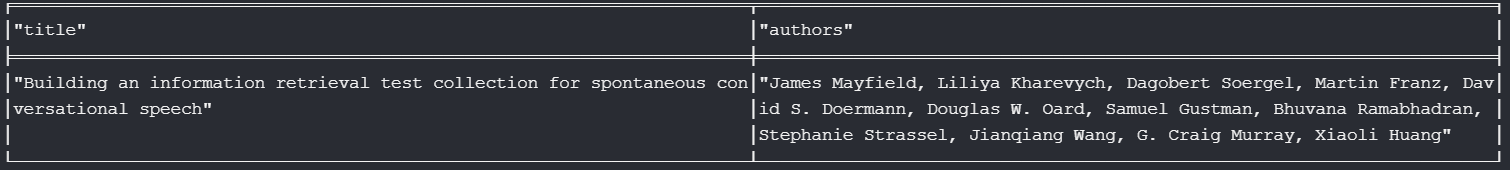
\includegraphics[width=1\textwidth]{query/query10.PNG}
\caption{Result: 1 record}
\label{fig:query10}
\end{figure}

\subsection{Query 11}
Find the article with most distinct university affiliations.\\
\textbf{Description:} We match all the \verb |WRITES| relationships (we could have used the \verb |WITH| keyword instead
of \verb |CALL|). This subquery returns all the distinct article-affiliation pairs. Then we group w.r.t. the article and
count its affiliations. We order the articles by counting in descending order and keep only the one with the greatest
number of different affiliations.
\textbf{Note:} this query complexity is of 2 nodes, but we decided to present it because of the relevance of the results.
\begin{lstlisting}[language=cypher, label=lst:cypher-example]
CALL{
    MATCH(article:Publication)<-[w:WRITES]-(author:Author)
    RETURN DISTINCT article, w.org as org
}
WITH  article, count(*) as n
ORDER BY n DESC LIMIT 1
RETURN  article.title,  n as AffiliationsCount
\end{lstlisting}
\begin{figure}[H]
\centering
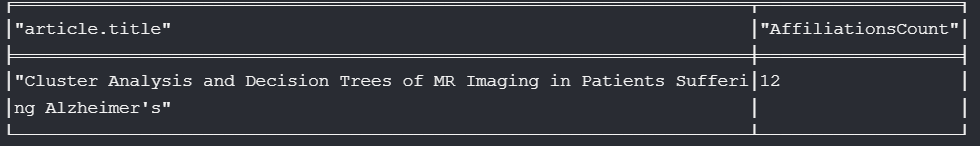
\includegraphics[width=0.7\textwidth]{query/query11.PNG}
\caption{Result: 1 record}
\label{fig:query11}
\end{figure}


\chapter{Conclusion}
Some interesting conclusions can be drawn from the development of this project: designing a Graph DB allows us to open a new
perspective in database creation. This technology enables an efficient visualization of the design choices and it is more
flexible than classical relational databases. \newline
Other very useful aspects of this project were the dataset pre-processing operation and the profiling that allows us to deal
with a real world problem of managing data.

\end{document}
